%%%%%%%%%%%%%%%%%%%%%%%%%%%%%%%%%%%%%%%%%%%%%%%%%%%%%%%%%%%%%%%%%%%%%%%%%%%%%%%%
%2345678901234567890123456789012345678901234567890123456789012345678901234567890
% 1 2 3 4 5 6 7 8
\documentclass[letterpaper, 10 pt, times, conference]{ieeeconf} % Comment this line out
% if you need a4paper
%\documentclass[a4paper, 10pt, conference]{ieeeconf} % Use this line for a4
% paper
\IEEEoverridecommandlockouts % This command is only
% needed if you want to
% use the \thanks command
%\overrideIEEEmargins
% See the \addtolength command later in the file to balance the column lengths
% on the last page of the document

\usepackage{graphicx}
\usepackage{multicol}
\usepackage{subfigure}
\usepackage{mathptmx} % use Times fonts if available on your TeX system
\usepackage{setspace}
\usepackage{algorithmicx}
\usepackage{algpseudocode}
% The following packages can be found on http:\\www.ctan.org
%\usepackage{graphics} % for pdf, bitmapped graphics files
%\usepackage{epsfig} % for postscript graphics files
%\usepackage{mathptmx} % assumes new font selection scheme installed
\usepackage{times} % assumes new font selection scheme installed
\usepackage{amsmath} % assumes amsmath package installed
\usepackage{amssymb} % assumes amsmath package installed
\title{\LARGE \bf
Locality-Based Dynamic Peer-to-Peer Communication for\\ Self-regulated Multi-robot Task Allocation
}
\author{ Md Omar Faruque Sarker and Torbj{\o}rn S. Dahl\\
%\thanks{This research has been funded by the Engineering and Physical Sciences Research Council (EPSRC), UK, grant reference EP/E061915/1.}%
Robotic Intelligence Lab, Newport Business School\\
University of Wales, Newport, Allt-yr-yn Campus\\ 
Allt-yr-yn Avenue, Newport, NP205XR, UK\\
{\tt\small Mdomarfaruque.Sarker@newport.ac.uk}\\ 
{\tt\small Torbjorn.Dahl@newport.ac.uk} 
}
%\author{Huibert Kwakernaak and Pradeep Misra% <-this % stops a space
%\thanks{This research has been funded by the Engineering and Physical Sciences Research Council (EPSRC), UK, grant reference EP/E061915/1.}% <-this % stops a space
%%\thanks{H. Kwakernaak is with Faculty of Electrical Engineering, Mathematics and Computer Science,
%% University of Twente, 7500 AE Enschede, The Netherlands
%% {\tt\small h.kwakernaak@autsubmit.com}}%
%%\thanks{P. Misra is with the Department of Electrical Engineering, Wright State University,
%% Dayton, OH 45435, USA
%% {\tt\small pmisra@cs.wright.edu}}%
%}
\begin{document}

\maketitle
\thispagestyle{empty}
\pagestyle{empty}
%%%%%%%%%%%%%%%%%%%%%%%%%%%%%%%%%%%%%%%%%%%%%%%%%%%%%%%%%%%%%%%%%%%%%%%%%%%%%%%%
\begin{abstract}
Distributed local communication is one of the essential means by which various social insects achieve their self-regulatory division of labour. However, applying this kind of decentralized communication technique in multi-robot task allocation (MRTA) is not as straight forward as a centralized one. From a robot controller's point of view, it is not easy to determine how often or how much dynamic peer-to-peer (P2P) communication is needed in order to maintain the convergence in MRTA. To deal with this issue, in this paper, we propose a locality based dynamic P2P communication model for achieving self-regulated MRTA. We present an implementation of this model on a typical multi-robot system (MRS) with two different local communication radii. We also compare this system with our baseline centralized communication based MRS in terms of convergence of MRTA, communication load, robot motions and their task specializations.  With our local communication model,  significant reductions in robot motions were observed. So it appears that this model can be used to minimize the overall energy usage of MRS. Additional results from these experiments suggest us that similar or better convergence of MRTA can be obtained by setting a smaller P2P communication radius where a robot locally exchanges signals with a minimum number of its nearby peers. Our experiments used 16 e-puck robots in a 2m X 2m arena.
%
\end{abstract}
%
%%%%%%%%%%%%%%%%%%%%%%%%%%%%%%%%%%%%%%%%%%%%%%%%%%%%%%%%%%%%%%%%%%%%%%%%%%%%%%%%
\section{INTRODUCTION}
\label{sec:intro}
Inspired from biological and various other social systems, robotic researchers have achieved self-regulated multi-robot task allocation (MRTA) using various forms of communications \cite{Bonabeau+1999,Labella}. Two basic forms of communications are: 1) direct or explicit communication and 2) indirect or implicit communication. {\em Direct communication} is an intentional communicative act of message passing that aims at one or more particular receiver(s) \cite{Mataric}. It typically exchanges information through physical signals. In contrast, indirect communication, sometimes termed as {\em stigmergic} in biological literature, happens as a form of modifying the environment (e.g., pheromone dropping by ants) \cite{Bonabeau+1999}. In ordinary sense, this is an observed behaviour and many robotic researchers call it as {\em no communication} \cite{Labella}. In order to avoid ambiguity,  by the term {\em self-regulated MRTA} (or {\em  MRTA} for short) we refer to those MRS where robots can  exhibit most common self-regulatory properties \cite{Bonabeau+1999} in their task-allocation process. Also in this paper,  by the term {\em communication}, we always refer to direct communication and we confine our discussion on MRTA within the context of direct communication only.\\
In order to pursue MRTA, robots can receive information from a centralised source \cite{Krieger} or from their local peers \cite{Agassounon}. In \cite{Sarker}, we reported a steady-state convergence of MRTA in a practical MRS using a centralized information source. This centralized communication system is easy to implement. It simplifies the overall design of a robot controller. However this system has disadvantage of a single point of failure and it is not scalable. The increased number of robots and tasks cause inevitable increase in communication load and transmission delay. Consequently, the overall system performance degrades. On the other hand, uncontrolled reception of information from decentralized or local sources is also not free from drawbacks. If a robot exchanges signals with all other robots (hereafter called as {\em peers}), it might get the global view of the system quickly and can select an optimal or near optimal task. This can produce a great improvement in overall performance of some types of tasks e.g., in area coverage \cite{Rutishauser}. But this is also not practical and scalable for a typically large MRS due to the limited communication and computational capabilities of robots and limited available communication bandwidth of this type of system.\\ 
A potential alternate solution to this problem can be obtained by decreasing the number of message recipient peers on the basis of a local communication radius ($r_{comm}$). This means that robots are allowed to communicate only with those peers who are physically located within a preset distance. When this strategy is used for sharing task information among peers, MRTA can be more robust and efficient \cite{Agassounon}. In this paper, we have presented a set of experimental results of MRTA with two values of $r_{comm}$: 0.5m and 1m. In case of the former one, we call the peers located within $r_{comm}$ as {\em nearby peers}. 
Along with a practical insight for selecting $r_{comm}$ value, various other design issues have been tackled in this paper. The recursion-free design of local communication channels is achieved by a dynamic publish/subscribe model of communication. This has been validated by using a state-of-the-art D-Bus \footnote{http://dbus.freedesktop.org/doc/dbus-specification.html} inter-process communication (IPC) technology in Linux.\\
Our contributions from this study are as follows. We present a locality based dynamic P2P communication model that achieves similar or better MRTA than its centralized counterpart. The reduction of robot motion is about half in this case and this tells us about the level of impact this local model can make on the energy efficiency of a MRS. The reduction of communication load in local model is also significant. Unlike a fixed communication frequency, the dynamic variation in communication frequency produced by our local model suggests us that local communication model should be preferred to a centralized one when robustness and scalability of MRTA is an important issue.\\
Rest of this paper is organized as follows. Section~\ref{sec:afm} presents attractive field model (AFM) \cite{Elsa} that allows us to implement an inter-disciplinary generic model of self-regulated division of labour as a multi-robot task allocation (MTRA) mechanism. Section~\ref{sec:comm-model} describes our local P2P communication model. Section~\ref{sec:impl} introduces our implementation of MRTA including the interactions between the hardware, software and communication modules. Section~\ref{sec:expt-design} presents the design of our experiments including specific parameters and observables. Section~\ref{sec:results} discusses our experimental results. Section~\ref{sec:bg} discusses related background works and section~\ref{sec:conc} draws conclusions.
%
%%%%%%%%%%%%%%%%%%%%%%%%%%%%%%%%%%%%%%%%%%%%%%%%%%%%%%%%%%%%%%%%%%%%%%%%%%%%%%%%
\section{Attactive Field Model (AFM)}
\label{sec:afm}
AFM provides us a generic framework for implementing self-regulatory MRTA. Here we briefly describe how this model gives our robots self-regulatory behaviours, particularly task-specialization, concurrency, flexibility and robustness. Interested readers should consult \cite{Elsa} for a general overview and \cite{Sarker} for our robotic implementation of AFM.
Let us consider a manufacturing shop floor scenario where N number of mobile robots are required to attend to M number of shop tasks spread over a fixed area A. Let these tasks be represented by a set of small rectangular boxes resembling to manufacturing machines. Let each task $j$ has an associated task-urgency $\phi_j$ that indicates its relative importance over time. If a robot attends to a task $j$ in x$^{th}$ time-step, value of $\phi_j$ will decreases by a small amount, $\delta_{\phi 1}$ in (x+1)$^{th}$ time-step. On the other hand, if a task has not been served by any robot in x$^{th}$ time-step, $\phi_j$ will increase by another small amount, $\delta_{\phi 2}$ in (x+1)$^{th}$ time-step. In order to complete a shop task $j$, a robot needs to reach within a fixed boundary of $j$, $D_j$. If a robot completes a task $j$ we say that it learns about it and this will increase robot's likelihood of selecting that task in next step. We call this variable affinity of a robot to that task as its sensitization $k_j$. If a robot does not do a task $j$ for some time, we say that it forgets about $j$ and $k_j$ has been decreased.\\
According AFM, all robots will establish attractive fields to all tasks due to the presence of a system-wide continuous flow of information. The strength of these attractive fields called stimulus will vary according to the distances between robots and tasks, task-urgencies and corresponding sensitizations of robots. This is encoded in Eq. \ref{eqn1}.
%\addtolength{\abovedisplayskip}{-15mm} 
\begin{multicols}{2} 
\begin{equation}
\small
S_{j}^{i} = tanh\{\frac{k_{j}^{i}}{d+\delta } \phi _{j}\}
\label{eqn1}
\end{equation}
\vspace*{0.25cm}
\begin{equation}
\small
P_{j}^{i} = \frac{S_{j}^{i}}{\sum_{j}^{}S_{j}^{i}}
\label{eqn2}
\end{equation}
\end{multicols}
%\addtolength{\belowdisplayskip}{-1mm} 
%\vspace{2mm}
Eq. \ref{eqn1} states that the stimuli of a robot $i$ to a particular task $j$, $S_{j}^{i}$ depends on robot's spatial distance $d$ to $j$, level of sensitization to that task ($k_{j}^{i}$) and perceived urgency of that task ($\phi _{j}$). We use a vary small value $\delta$ in Eq. \ref{eqn1} to prevent division by zero. The probability of selecting each task has been determined by a probabilistic method outlined in Eq. \ref{eqn2} \cite{Elsa}. 
AFM ensures concurrency of a self-regulatory system by specifying at least two task options: 1) doing a task and 2) doing no task. In robots, the latter can be be treated as random walking. So in any time-step a robot will choose from M+1 tasks. Let $T_a$ be the allocated time to accomplish a task. If a robot can enter inside the task boundary, $r_{task}$ within $T_a$ time it waits there until $T_a$ elapsed. Otherwise it will select a different task. 
%%%%%%%%%%%%%%%%%%%%%%%%%%%%%%%%%%%%%%%%%%%%%%%%%%%%%%%%%
\section{Locality-based P2P Communication Model}
\label{sec:comm-model}
%%
\begin{figure}
\centering
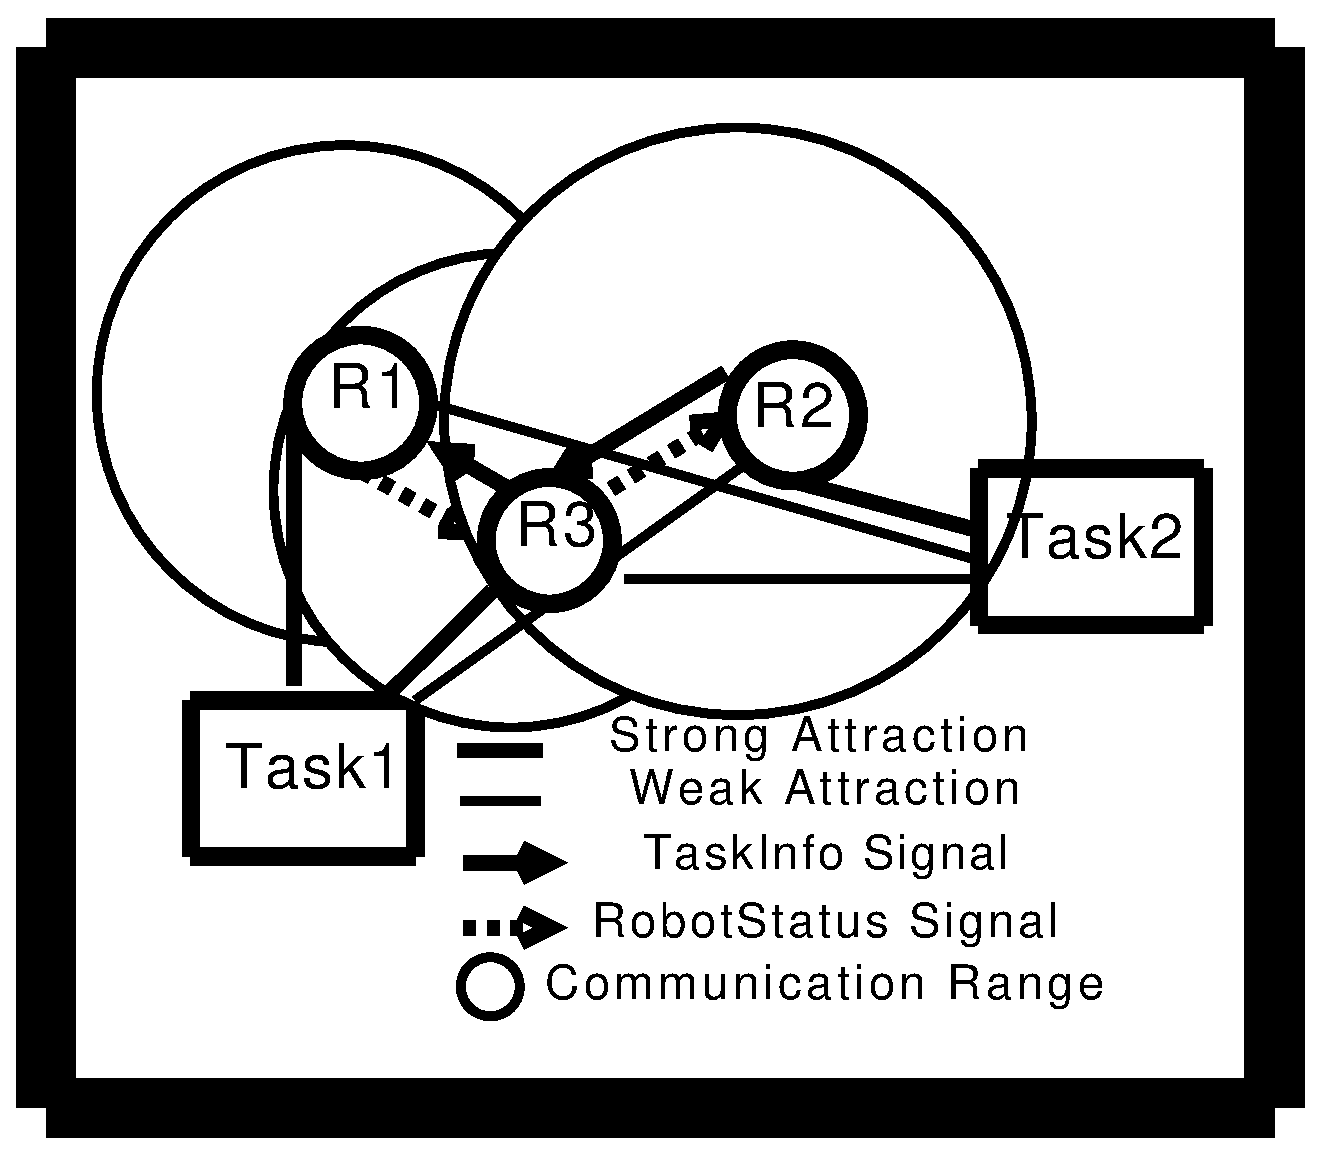
\includegraphics[height=4cm]{../dia-files/LocalComm}
% figure caption is below the figure
%\vspace*{0.20cm}
\caption{Local communication model}
\label{fig:lcm} % Give a unique label
\end{figure}
%%
\subsection{Characteristics}
Our communication model relies on the local P2P communications among robots. Here there is no centralized server to disseminate information but each robot can communicate to its nearby peers within a certain communication radius, $r_{comm}$. Here by $r_{comm}$, we assume that within this distance robots can exchange communication signals reliably without any significant loss of information. A robot $R_1$ is a {\em peer} of robot $R_2$, if spatial distance between $R_1$ and $R_2$ is less than its $r_{comm}$. As shown in Fig. \ref{fig:lcm}, local communication can also give robots similar task information as in centralized communication mode. It shows that it is not necessary for each robot to communicate with every other robot to get information on all tasks. Since robots can random walk and explore the environment we assume that for a reasonably high robot to space density, all task will be known to all robots after an initial exploration period. In order to update the urgency of a task, robots can estimate the number of robots working on a task in many ways: such as, by using their sensory perception (e.g., camera), by doing local P2P communication and so on. In Fig. \ref{fig:lcm} we have shown that robots exchange both task information and self status signals to peers.\\
We characterize our communication model in terms of three fundamental issues: 1) message content ({\em what to communicate}) 2) communication frequency ({\em when to communicate}) and 3) target recipients ({\em with whom to communicate}) \cite{Gerkey}. In a typical MRS, message content can be categorized into two types: 1) state of each individual robot and 2) target task (goal) information \cite{Balch}. The latter can also be subdivided into two types: 1) an individual robot's target task information and 2) information of all available tasks found in the system. Regarding the first issue, our communication model is open. Robots can communicate with their peers with any kind of message. Our model addresses the last two issues very specifically. Robots communicate only when they meet their peers within a certain communication radius ($r_{comm}$). Although in case of an environment where robots move relatively faster the peer relationships can also be changed dynamically. But this can be manipulated by setting the signal frequency and robot to space density to somewhat reasonably higher value. In terms of target recipients, our model differs from a traditional publish/subscribe communication (PSC) model by introducing the concept of dynamic subscription. In a traditional PSC model, subscription of messages happens prior to the actual message transmission. In that case prior knowledge about the subjects of a system is necessary. But in our model this is not necessary as long as all robots uses a common addressing convention for naming their incoming signal channels. In this way, when a robot meets with another robot it can infer the address of this peer robot's channel name by using a shared rule. A robot is thus always listening to its own channel for receiving messages from its potential peers or message publishers. On the other side, upon recognizing a peer a robot sends a message to this particular peer. So here neither it is necessary to create any custom subject namespace (e.g., \cite{Gerkey}) nor we need to hard-code information in each robot controller about the knowledge of their potential peers {\em a priori}. Subscription is done automatically based on their respective $r_{comm}$.
%
\subsection{Implementation Algorithm}
Our local communication model has three major aspects: 1) local sensing of peers (and optionally tasks), 2) listening to peer signals and 3) emitting signals for peers. Here we present a typical implementation.
Let N be the set of robots. At time step q, a robot $i$ that can receive $h_{i,q}$ information by listening to its incoming channel $L_i$. Let M be the set of tasks. Each task $j$ has an associated information $H_j$. It encodes the necessary properties of tasks, such as their locations, urgencies etc. Each task $j$ also has a task perception radius $r_{task}$ such that if a robot comes within this radius at time step q it can perceive current value of $H_{j,q}$. Let at time step q, robot $i$ has its own task information $G_{i, q}$ that has been perceived and listened from its peers. Let $r_{comm}$ be the communication radius of each robot. Let at time step q, $P_{p, q}^{i}$ be a set of peers of $i$ that are within $r_{comm}^{i}$. Let $E_{p, q}^{i}$ be its active signal emission channels. Algorithm 1
implements our proposed dynamic P2P communication.\\  

\textbf{\small Algorithm 1: Locality based Dynamic P2P Communication}
\begin{algorithmic}[1]
\label{alg:p2p-comm}
\State $\textbf{Initialization:}$
\State $id \gets robotid$
\State $r_{comm} \gets r_1$
\State $r_{task} \gets r_2$
\State $pose[id] \gets (0, 0, 0)$
\State $G[id], ~P[id], ~L[id], ~E[~] \gets 0$
\State $\textbf{Loop:}$
\State $pose[id] \gets (x, y, \theta)$
% PERCEPTION of TASK
\If {$pose[id] \in U(pose[k],~ r_{task}^{k}), (k = 0, 1, …., M-1)$} 
\State $G[id] \gets G[id] ~\cup ~ H_k$
\EndIf
% P2P Interaction, listen signal
\If {$pose[id] \in V(pose[k],~ r_{comm}^{k}), (k = 0, 1, …., N-1, k\neq id )$} 
\State $P[id] \gets P[id] ~ \cup ~ k$
\State $h_k \gets W(E[k],~ L[id])$
\State $G[id] \gets G[id] ~ \cup ~ h_k$
\EndIf
% P2P Interaction, emit signal
\ForAll {$ k \in P[id], (k = 0, 1, …., N-1, k\neq id)$}
\State $ W(E[id],~L[k]) \gets G[id]$
\EndFor
\State $P[id] \gets 0$
\State $\textbf{Loop again}$
\end{algorithmic}
%\addtolength{\floatsep}{-25mm}
%
From Algorithm 1, we see that a robot controller is initialized with its specific robot-id and default values of $r_{comm}$ and $r_{task}$. We assumed that these values are same for all robots and for all tasks respectively.
Initially a robot has no information about tasks. It has neither listened nor transmitted any information yet. Upon initialization, robot determines its current pose and evaluates a function $U(pose,~ r_{task})$ that helps it to perceive information of a nearby task. This is not strictly necessary as this information can be available from alternate sources. In second step, robot senses its nearby peers by evaluating $V(pose,~ r_{comm})$ and start filling the list of peers $P$ by their id. The signal exchange with a peer is denoted by a communication function $W(emitter,~listener)$. So by listening to a peer signal, it receives task information $h$ and aggregates this $h$ with its own task info $G$. In last step, robot emits its task information to its peers stored in $P$. Finally it erases all values of $P$ and repeat this loop. 
%
%%%%%%%%%%%%%%%%%%%%%%%%%%%%%%%%%%%%%%%%%%%%%%%%%%%%%%%%%%%%%%%%%%%%%%%%%%%%%%%%
\section{Implementation}
\label{sec:impl}
\begin{figure}
\centering
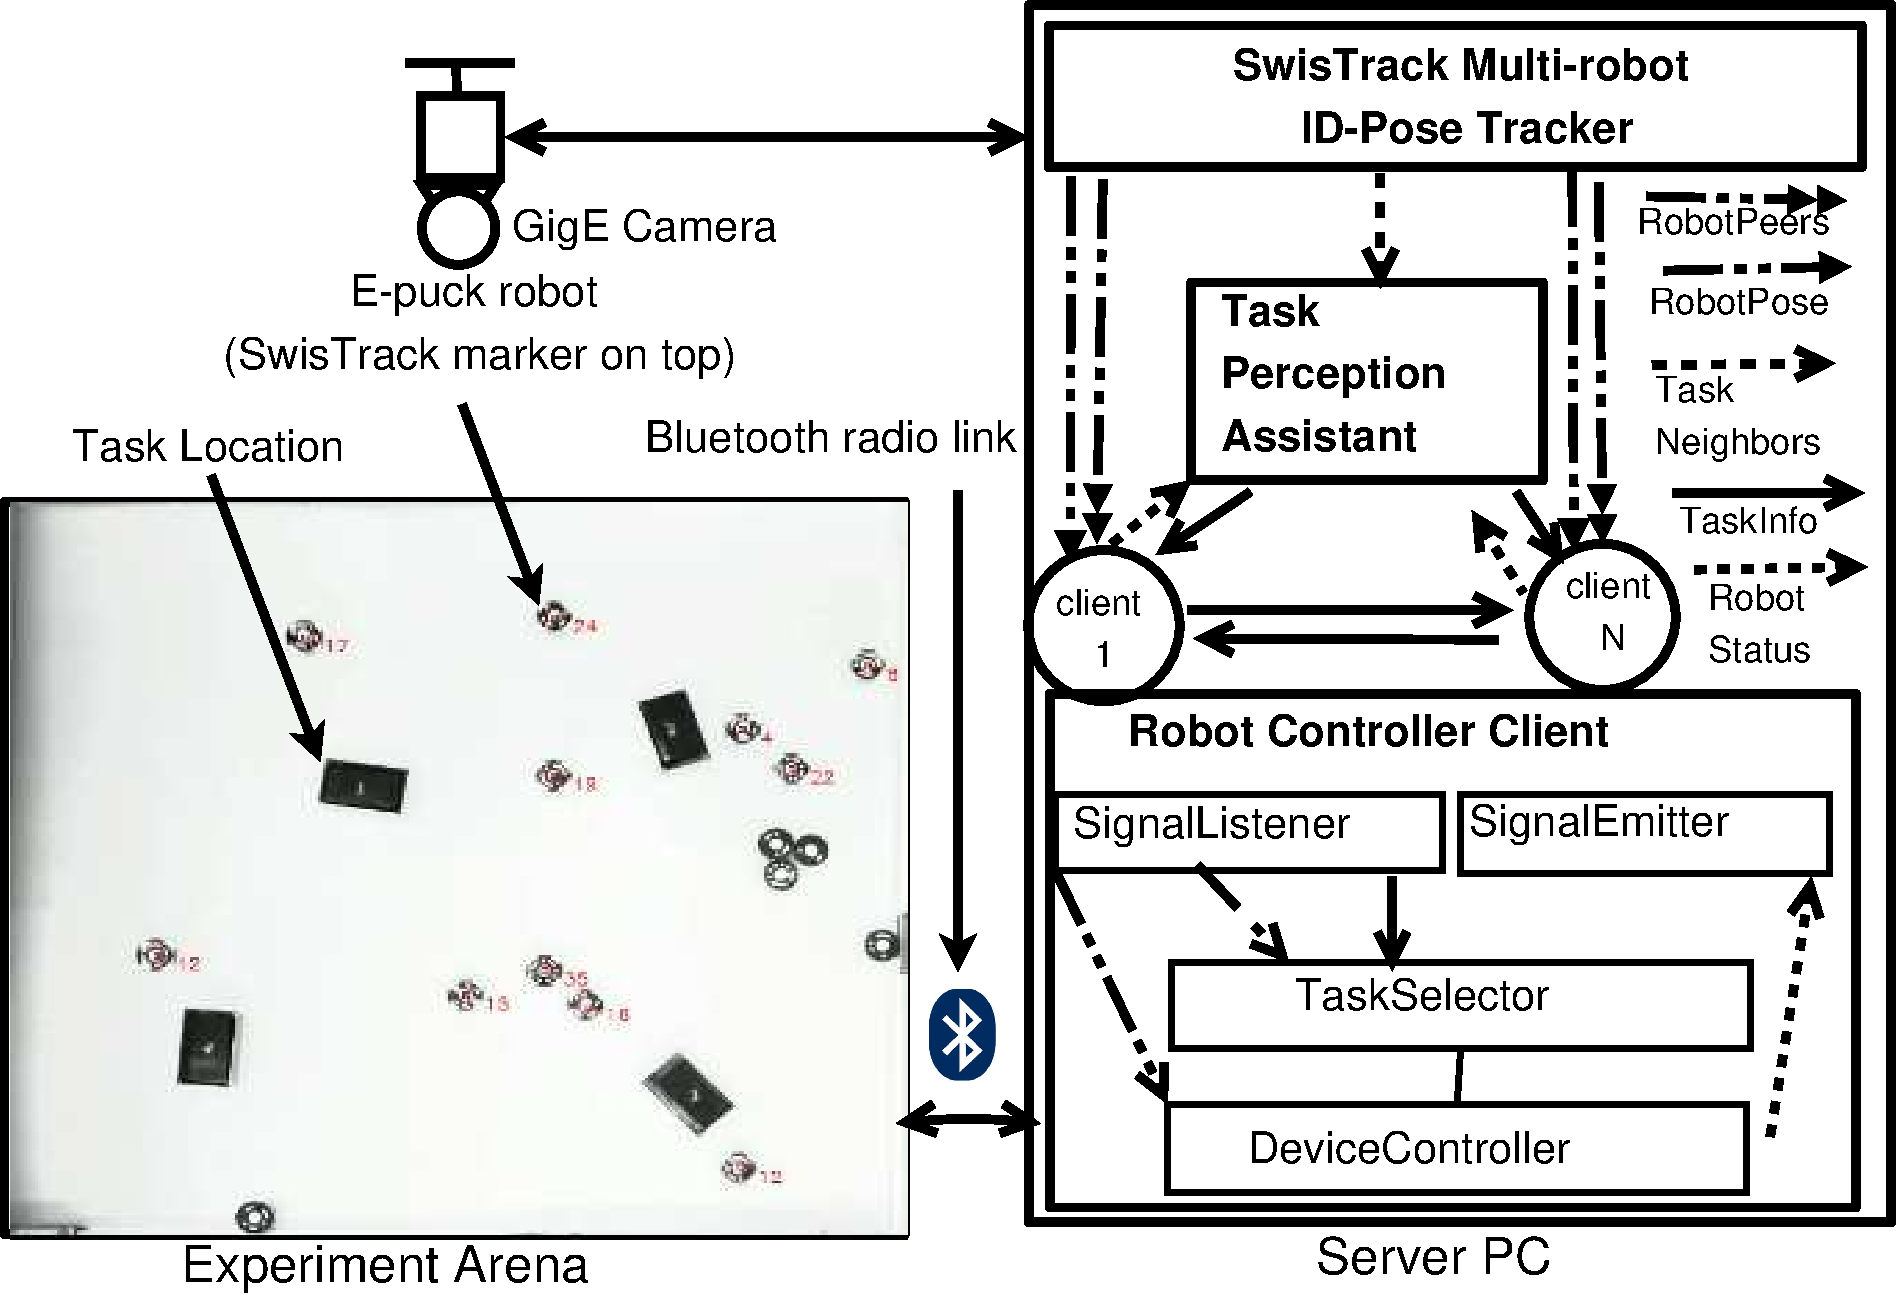
\includegraphics[width=9cm, angle=0]
{../dia-files/RIL-Expt-Setup2}
%figure caption is below the figure
\caption{\small Hardware and software setup}
\label{fig:setup} % Give a unique label
\end{figure}
We have developed a system where up to 40 E-puck robots \cite{Epuck} can operate together according to the generic rules of the AFM. As shown in Fig. \ref{fig:setup} (right), our software system consists of a multi-robot tracking system, a task perception assistant (TPA) and robot controller clients (RCC). Here at first we have presented the design of our communication system. Then we have discussed about our specific MRS implementation. 
%%%
\subsection{Our communication system}
As shown in Fig. \ref{fig:setup}, RCCs disseminate task information to each other by \textit{TaskInfo} D-Bus signal. The contents of task information are physical locations of tasks and their urgencies. However as our robots are incapable of sensing task directly. So it relies on TPA for actual task location and urgency. When a robot $i$ comes within $r_{task}$ of a task $j$, SwisTrack reports it to TPA (by {\em TaskNeighbors} signal) and TPA then gives it current task information $H_j$ to $i$ (by {\em TaskInfo} signal).
TPA has another interface for catching feedback signals from robots. The \textit{RobotStatus} signal can be used to inform TPA about a robot's current task id, its device status and so on. TPA uses this information to update relevant part of task information such as, task-urgency. This up-to-date information is encoded in next TaskInfo signal.\\
%In Fig. \ref{fig:lcm} an initial configuration of our communication system has been presented. Upon receiving an initial TaskInfo signal from TPA, robot $R_3$ has shown strong attraction towards $Task1$ and robot $R_2$ has shown strong attraction toward $Task2$. However $R_1$ receives information about both tasks through its peer $R_3$ and shows strong attraction towrads Task1. These can be inferred from Eq. \ref{eqn1} that says if the initial task urgencies and sensitizations for all tasks are same, a robot will strongly be attracted towards a task that is relatively closer to it.
\subsection{Our current implementation}
In order to track all robots real-time we have used SwisTrack \cite{SwisTrack}, a state of the art open-source, multi-agent tracking system, with a16-megapixel overhead GigE camera. This set-up gives us the position, heading and id of each of the robots at a frequency of 1. The interaction of the hardware and software of our system is illustrated in Fig. \ref{fig:setup}. \\
For IPC, we have used D-Bus technology. %\footnote{http://dbus.freedesktop.org/doc/dbus-specification.html}. 
We have developed an IPC component for SwisTrack (hereafter called as \textit{SwisTrack D-Bus Server}) that can broadcast id and pose of all robots in real-time over our server's D-Bus interface.\\
Apart from SwisTrack, we have implemented two major software modules: {\em Task Perception Assistant (TPA)} and {\em Robot Controller Client (RCC)}. They are developed in Python with its state of the art \textit{Multiprocessing} \footnote{http://docs.python.org/library/multiprocessing.html} module. This python module simplifies our need to manage data sharing and synchronization among different sub-processes. As shown in Fig. \ref{fig:setup}, RCC consists of four sub-processes. {\em SignalListener} and {\em SignalEmitter}, interface with SwisTrack D-Bus Server and TPA. {\em TaskSelector} implements AFM guidelines for task selection . {\em DeviceController} moves a robot to a target task. Bluetooth radio link is used as a communication medium between a RCC and a corresponding E-puck robot. 
%
%%%%%%%%%%%%%%%%%%%%%%%%%%%%%%%%%%%%%%%%%%%%%%%%%%%%%%%%%%%%%%%%%%%%%%%%%%%%%%%%%
\section{Experiment Design}
\label{sec:expt-design}
In this section, we have described the design of parameters and observables of our experiments.
These experiments are designed to validate AFM by testing the occurrence of convergent MRTA. Table \ref{table:params} lists a set of essential parameters of our experiments. 
%
\begin{table}
\caption{Experimental parameters}
\label{table:params}
\begin{center}
\begin{tabular}{|l||c|}
\hline Parameter & Value\\
\hline Total number of robots ($N$) & 16\\
\hline Total number of tasks ($M$) & 4\\
\hline Experiment area ($A$) & 4 $m^2$\\
\hline Intial task urgency ($\Phi_{INIT}$) & 0.5\\
\hline Task urgency increase rate ($\Delta\phi_{INC}$) & 0.005\\
\hline Task urgency decrease rate ($\Delta\phi_{DEC}$) & 0.0025\\
\hline Intial sensitization ($K_{INIT}$) & 0.1\\
\hline Sensitization increase rate ($\Delta k_{INC}$) & 0.03\\
\hline Sensitization decrease rate ($\Delta k_{DEC}$) & 0.01\\
\hline A very small distance ($\delta$)& 0.000001\\
\hline Task info update interval ($\Delta TS_{u}$) & 5s\\
\hline Task info signal emission interval ($ \Delta TS_{e}$)& 2.5s\\
\hline Robot's task time-out interval ($\Delta RT_{to} $)& 10s\\
\hline
\end{tabular}
\end{center}
\end{table}
\subsection{Parameters}
We intend to have a setup that is relatively complex, i.e., a high number of robots and tasks in a large area, but with a high probability of convergence. The following criteria shows our rationale behind our selected parameters.
%
\begin{itemize}
\item Robots should be capable of moving at a reasonably high speed (e.g., $\geq 4 cm/s$) without interfering to each other very much.
\item Tasks density should be as least one task per square meter.
\item Host PC to robot communication should be as dedicated and stable as possible.
\item No task should be left unattended completely for a long time (e.g., $\geq 300s $).
\end{itemize}
%
When many Bluetooth devices talk to a single Bluetooth adapter, communication delays become very frequent due to the fact that each device gets a guaranteed turn to communicate \cite{Bluetooth}. After some initial testing, we found a stable server configuration with 8 Bluetooth adapters, i.e., one Bluetooth adapter is used to communicate with two robots. This limits us to set the total number of robots to 16. Also we found that after about 35-40 minutes from the start of our experiments some of robots fail to get the access to their designated Bluetooth adapters. So we limit the length of our experiments to 40 minutes. We expect that this limitation would be removed by distributing Bluetooth adapters among multiple server PCs.\\ 
The diameter of the marker of our E-puck robot is 8cm. So, if we put 4 robots in an area of one square meter, this will give us a robot-occupied-space to free-space ratio of about 1:49 per square meter. We have found that this ratio is reasonable to allow the robots to move at a speed of 7.5 cm/sec without much interference to each other. We randomly placed four 18.5 cm x 11.5 cm rectangular boxes as a shop task in our experiment arena. They were about one meter apart from each other.\\
The initial values of task urgencies can be set to any value as long as they are same for all tasks. We choose a limit of 0 and 1, where 0 means no urgency and 1 means maximum urgency. Same applies to sensitisation as well, where 0 means no sensitisation and 1 means maximum sensitisation. We choose a default sensitization value of 0.1 for all tasks. Our rationale behind selecting task urgency and sensitisation change rates can be found in \cite{Sarker}.
%The following relationships are maintained for selecting task-urgency and sensitization parameters.
%
%\begin{equation}
%\Delta\phi_{INC} = \frac{\Delta\phi_{DEC} \times N}{2 \times M}
%\label{eqn:task-urgency}
%\end{equation}
%%
%\begin{equation}
%\Delta k_{DEC} = \frac{\Delta k_{INC}} {M - 1} 
%\label{eqn:sensitization}
%\end{equation}
%%
%Eq. \ref{eqn:task-urgency} establishes the fact that task urgency will increase at a higher rate than that of its decrease. As we do not like to keep a task left unattended for a long time we choose a higher rate of increase of task urgency. This difference is set on the basis of our assumption that at least half of the expected number of robots (ratio of number of robots to tasks) would be available to work on a task. \\
%Eq. \ref{eqn:sensitization} suggests that the learning will happen much faster than the forgetting. The difference in these two rates is based on the fact that faster leaning gives a robot more chances to stick on to it. The exact ratio of learning and forgetting is related here by the fact that if a robot works on a task it learns about it and forgets about the rest. 
\subsection{Observables}
We have defined a set of observables to benchmark our implementation. They are briefly explained here.\\
\textbf{Changes in task-urgencies ($\Delta \Phi$): }
In our experiments, urgency of each task in each step has been logged. From the above design of task urgency, we can see that if a task is not served by any robot for 100 consecutive steps (500s), urgency of that task will reach from 0.5 to its maximum value 1.0. On the other hand, if a task is served by only one robot for 200 consecutive steps (1000s) urgency of that task will be 0. But in real experiment, it is more likely that more than one robot will serve a task. So urgency of a task will decrease $\Delta\phi_{DEC}$ times number of working robots on that task (based on AFM guidelines \cite{Elsa}). The overall changes in task urgencies will show the convergence behaviour of our system.\\
\textbf{Changes in robot sensitizations ($\Delta K$): }
According AFM, as robots will do tasks they will specialize on each task by increasing or decreasing sensitizations (learning and forgetting). From our above design, we can see that if a robot starts doing a task with an initial sensitization of 0.1 and it repeatedly does it for 30 consecutive steps, sensitization will reach to 1. Thus by logging the sensitization data of each robots we will be able to comment on task specializations of robots.\\
\textbf{Changes in robot motions ($\Delta U$): }
As we might guess that initially the task urgencies will be relatively higher for all tasks so robots will need to do a lot of movements by switching from one task to another. But as the system approaches to converge overall robot motions will be decreased. In order to observe this phenomena we log the pose of robots in every time step.\\
\textbf{D-Bus Signals emitted by Task server ($S_f$):} 
In order to measure the communication load on our communication system we are also interested to log P2P TaskInfo D-Bus signals. Since the emission of signals happens asynchronously it is more likely that the overall communication load on the system will vary over time. This is contrary to the centralized communication where communication load is almost constant over time.
%%%%%%%%%%%%%%%%%%%%%%%%%%%%%%%%%%%%%%%%%%%%%%%%%%%%%%%%%%%%%%%%%%%%%%
\section{Results and Discussions}
\label{sec:results}
%%
In this section we have presented our experimental results. We ran those experiments for about 40 minutes and averaged them from three iterations. For comparison purposes, here we present some of the results of our baseline experiments in centralized communication mode. Details can be found in \cite{Sarker}.\\
%%% raw urgencies
\begin{figure}
\centering
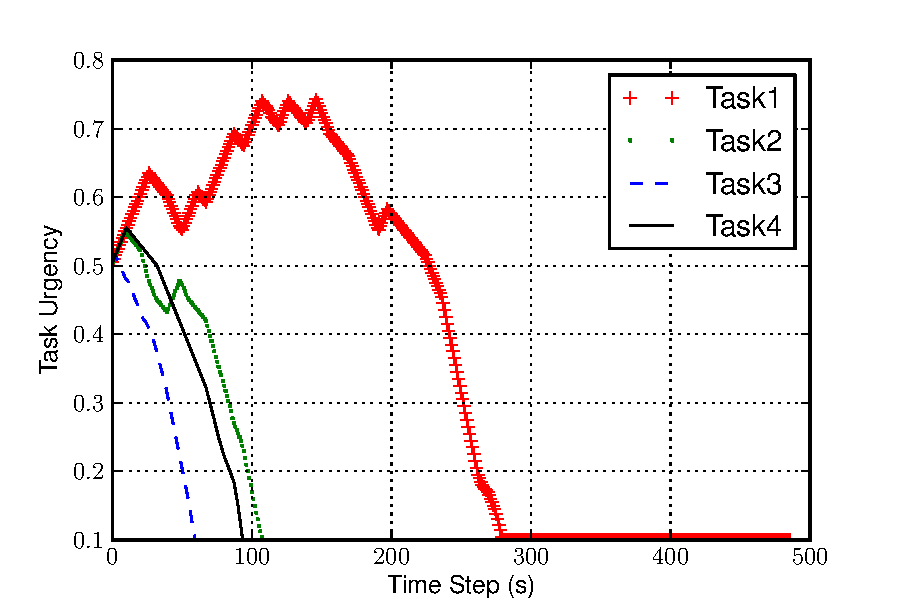
\includegraphics[height=5cm]
{images/local-500cm/PlotUrgencyLog-2010Feb15-171017}
%figure caption is below the figure
\caption{\small Task urgencies observed in local mode $r_{comm}$=0.5m}
\label{fig:raw-urgencies} % Give a unique label
\end{figure}
%%%
Fig. \ref{fig:raw-urgencies} shows the dynamic changes in task urgencies.
In order to describe our system's dynamic behaviour holistically we analyse the changes in task urgencies over time. Let $ \phi_{j, q}$ be the urgency of a task $j$ at $q^{th}$ step. In $(q+1)^{th}$ step, we can find the change of urgency of task $j$ :\\
\begin{equation} 
\small
\delta \phi_{j, q+1} = ( \phi_{j, q+1} - \phi_{j, q}) 
\end{equation}
So we can calculate the sum of changes in urgencies of all tasks at $(q+1)^{th}$ step:
\begin{equation} 
\small
\Delta \Phi_{j, q+1} = \sum_{j=1}^{M} \delta \phi_{j, q+1} 
\label{eqn:Delta-Phi}
\end{equation}
Fig. \ref{fig:urgency-convergence} plots this sum of changes of task urgencies by a dashed line. If we consider the absolute change over a window of time $w$ in the following equation, we can describe the overall changes of our systems in both positive and negative directions.
%
\begin{equation}
\small
\Delta \Phi_{jw, q+1} = \sum_{j=0}^{w-1} \left | \Delta \Phi_{q+j} \right |
\end{equation}
%
In order to find convergence in MRTA we have calculated the sum of absolute changes in task urgencies over a window of 2 consecutive steps (100s). This is plotted in solid line in Fig. \ref{fig:urgency-convergence}. Note that we scale down the time steps of this plot by aggregating the values of 10 consecutive steps (50s) of Fig. \ref{fig:raw-urgencies} into a single step value.
From Fig. \ref{fig:urgency-convergence} we can see that initially the sum of changes of task urgencies are towards negative direction. This implies that tasks are being served by a high number of robots. When the task urgencies stabilize near zero the fluctuations in urgencies become minimum. Since robots chose tasks stochastically, there will always be a small changes in task urgencies. A potential convergence point is located by considering the persistence existence of the value of $\Delta \Phi_{jw, q+1}$ below a threshold 0.1. Tn Fig. \ref{fig:urgency-convergence} this convergence happens near step 23 or after 1150s from the beginning of our experiments. This implies that from this point of time and onwards, changes of our system's behaviour remain under a small threshold value.\\
Using this same criteria, we can find that in local communication experiment convergence happens after step 14 in case of $r_{comm}$=0.5m (Fig. \ref{fig:local50cm-convergence}) and after step 29 in case of $r_{comm}$=1m (Fig. \ref{fig:local1m-convergence}).\\ 
%%%%
%%%% Centralized expt
\begin{figure*}
\begin{minipage}[t]{0.5\linewidth}
\centering
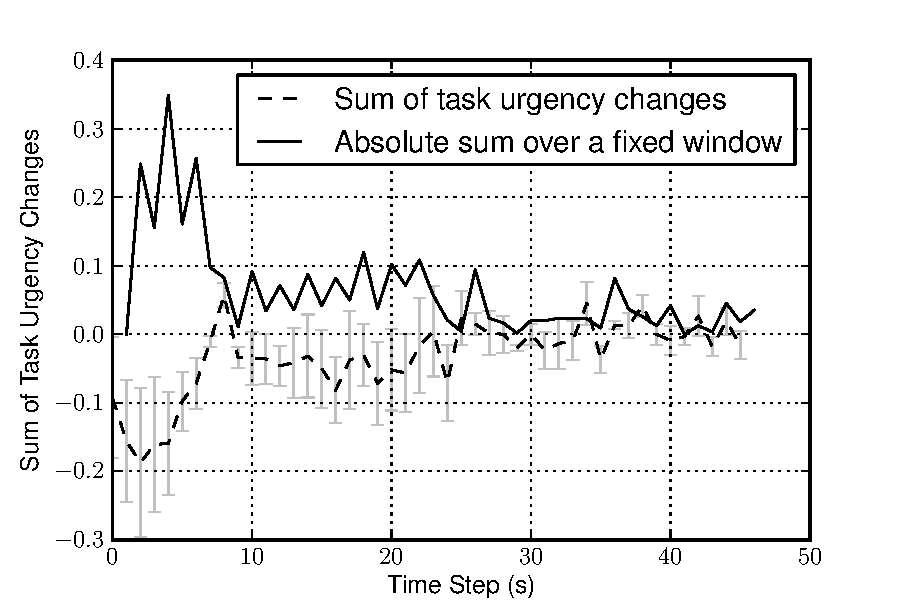
\includegraphics[height=5cm,width=3in]{images/global/TaskUrgencyConvergence-step2-th-p1}
\caption{\small Convergence of task urgencies in centralized mode}
\label{fig:urgency-convergence} % Give a unique label
\end{minipage}
\hspace{0.5cm}
\begin{minipage}[t]{0.5\linewidth}
\centering
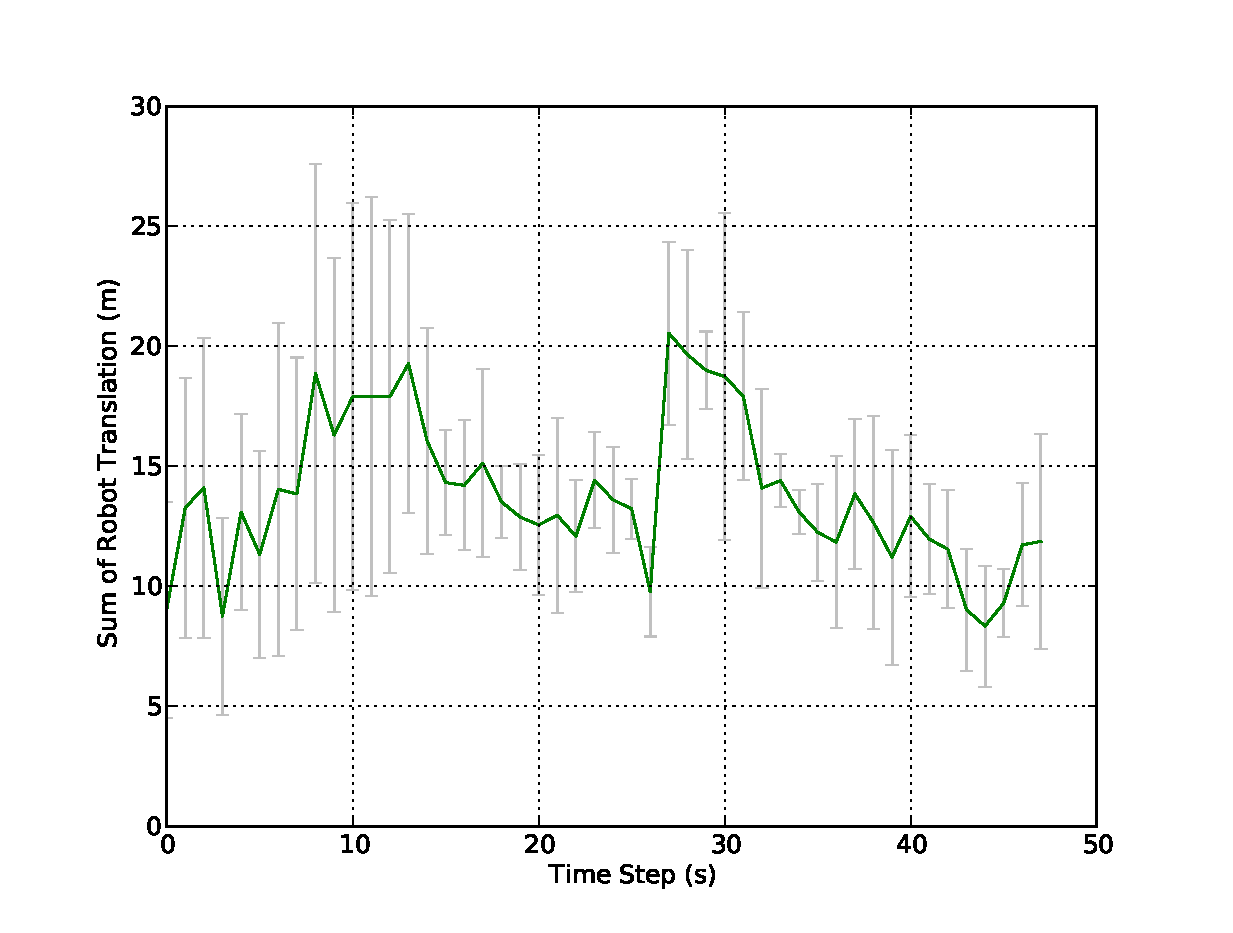
\includegraphics[height=5cm,width=3in]{images/global/DeltaTranslationStat}
\caption{\small Sum of translations of all robots in centralized  mode }
\label{fig:translation-stat} % Give a unique label
\end{minipage}
\end{figure*}
%%
%%
%%%%% Task Urgency Convergence/ Traslation local 50cm
\begin{figure*}
\begin{minipage}[t]{0.5\linewidth}
\centering
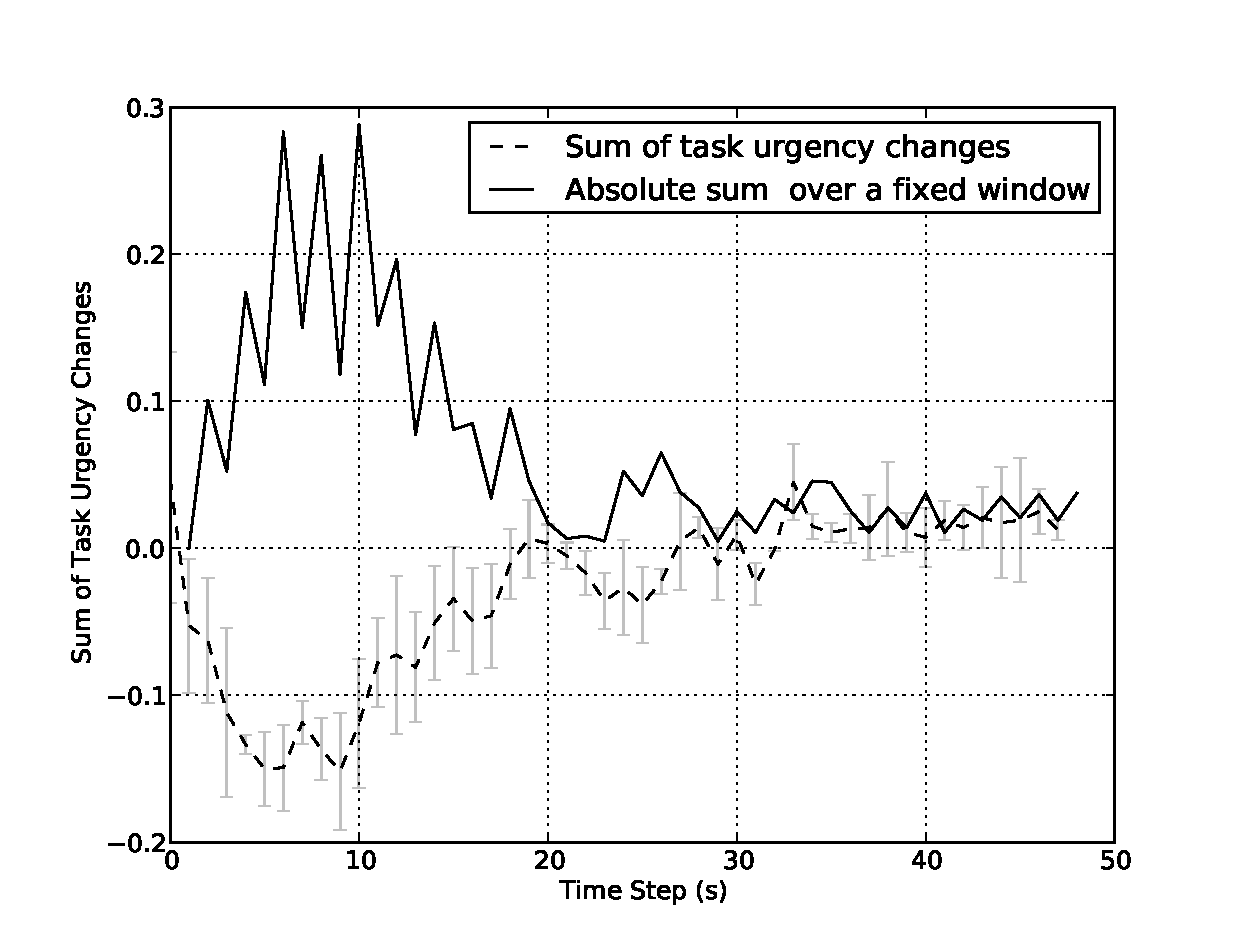
\includegraphics[height=5cm,width=3in]
{images/local-500cm/Local50cm-TaskUrgencyConvergence}
%figure caption is below the figure
\caption{\small Convergence of task urgencies in local mode $r_{comm}$=0.5m}
\label{fig:local50cm-convergence} % Give a unique label
\end{minipage}
\hspace{0.5cm}
\begin{minipage}[t]{0.5\linewidth}
\centering
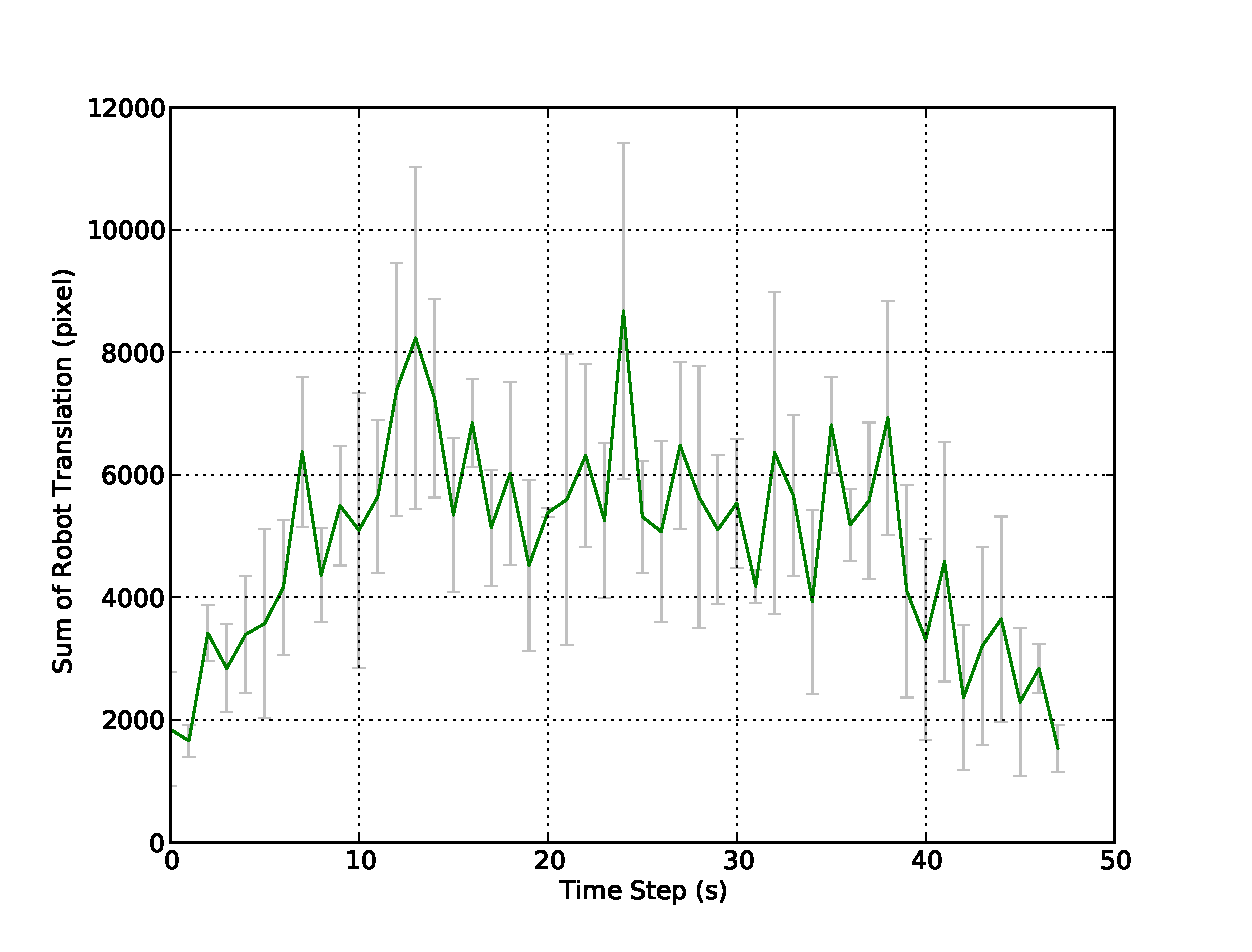
\includegraphics[height=5cm,width=3in]
{images/local-500cm/DeltaTranslationStat}
%figure caption is below the figure
\caption{\small Sum of translations of all robots in local mode $r_{comm}$=0.5m }
\label{fig:local50cm-tr} % Give a unique label
\end{minipage}
\end{figure*}
%%
%%%%% Task Urgency Convergence/ Traslation local local 1m %%%
\begin{figure*}
\begin{minipage}[t]{0.5\linewidth}
\centering
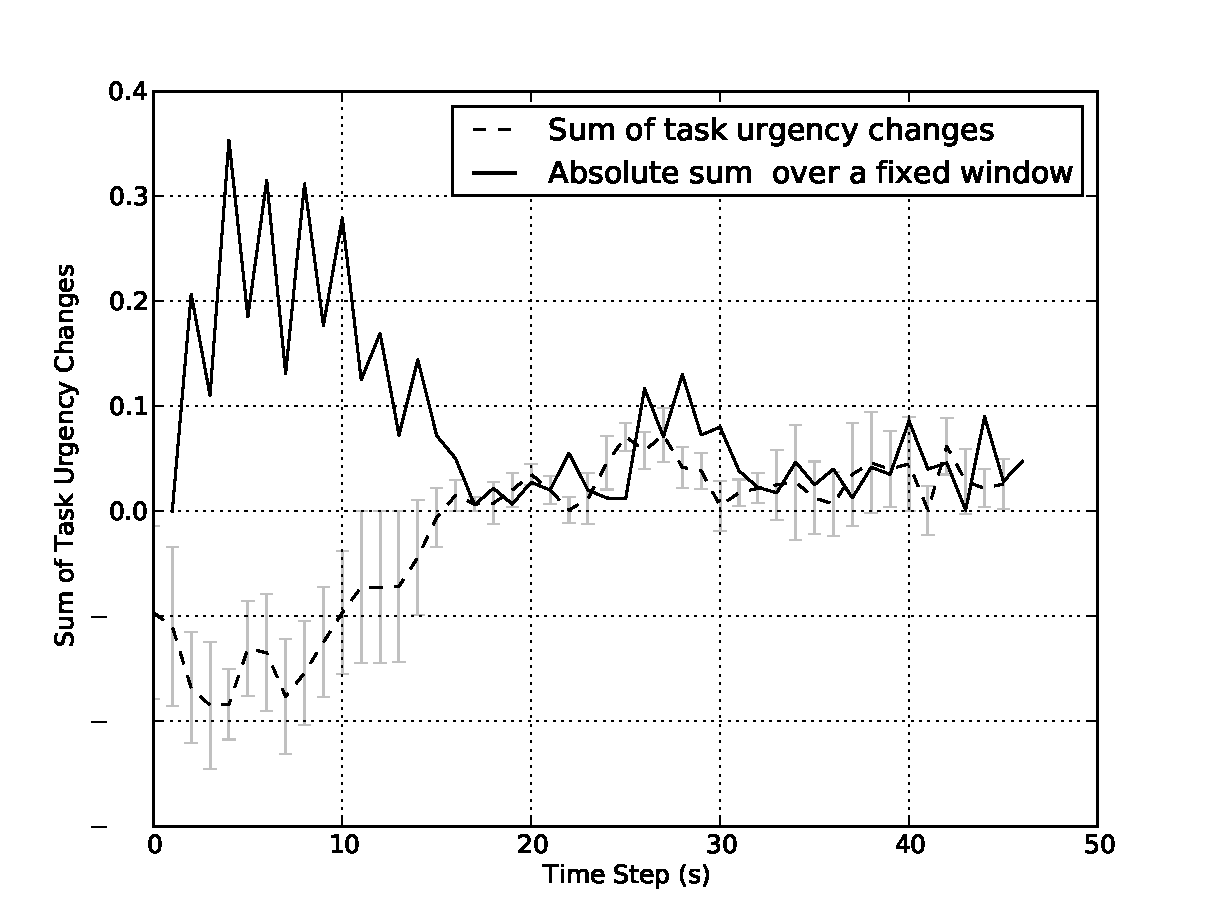
\includegraphics[height=5cm,width=3in]{images/local-1m/TaskUrgencyConvergence-1m}
\caption{\small Convergence of task urgencies in local mode $r_{comm}$=1m}
\label{fig:local1m-convergence} % Give a unique label
\end{minipage}
\hspace{0.5cm}
\begin{minipage}[t]{0.5\linewidth}
\centering
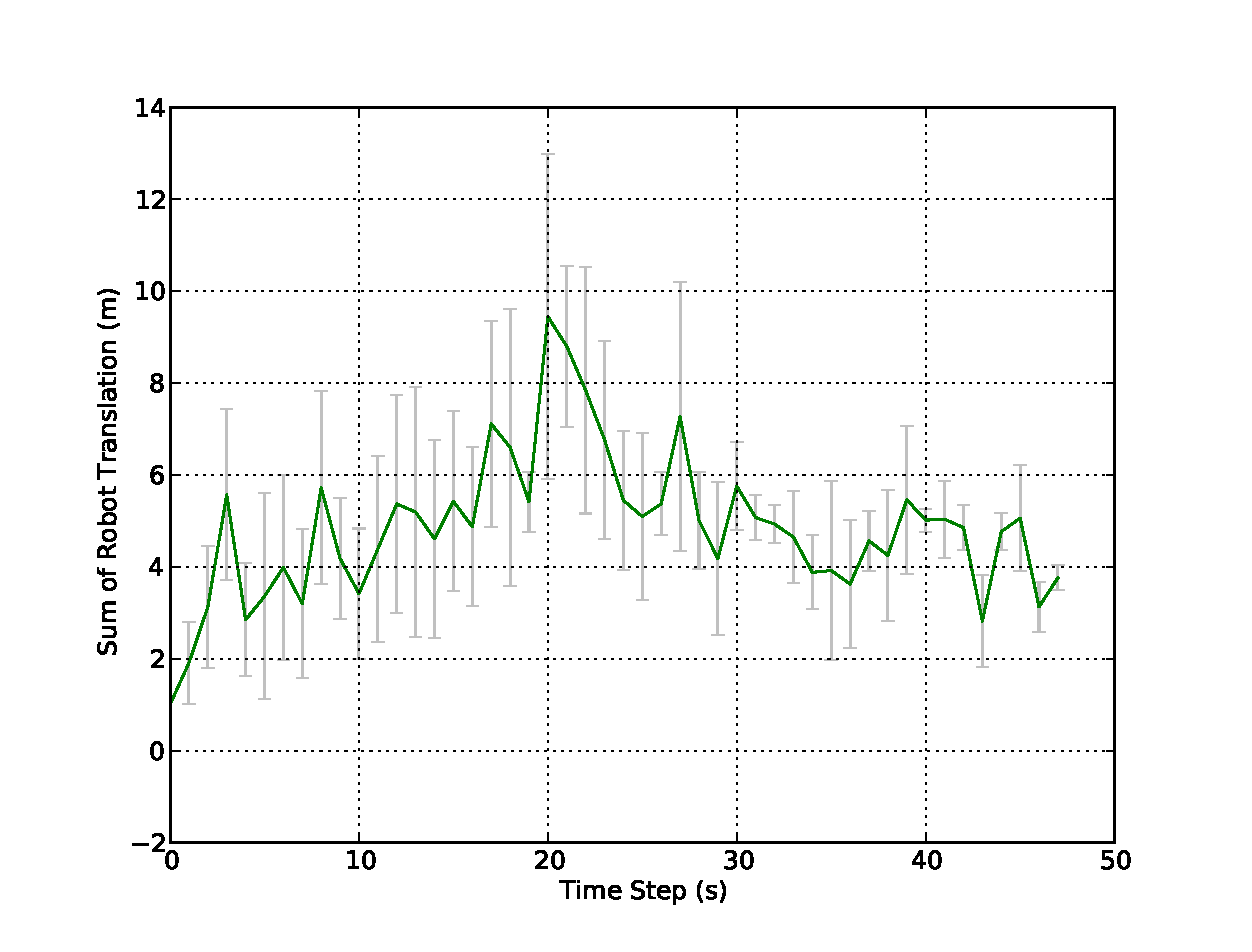
\includegraphics[height=5cm,width=3in]{images/local-1m/DeltaTranslationStat}
\caption{\small Sum of translations of all robots in local mode $r_{comm}$=1m }
\label{fig:local1m-tr} % Give a unique label
\end{minipage}
\end{figure*}
%%
%%% Sensitization%%%
\begin{figure*}
\begin{minipage}[t]{0.5\linewidth}
\centering
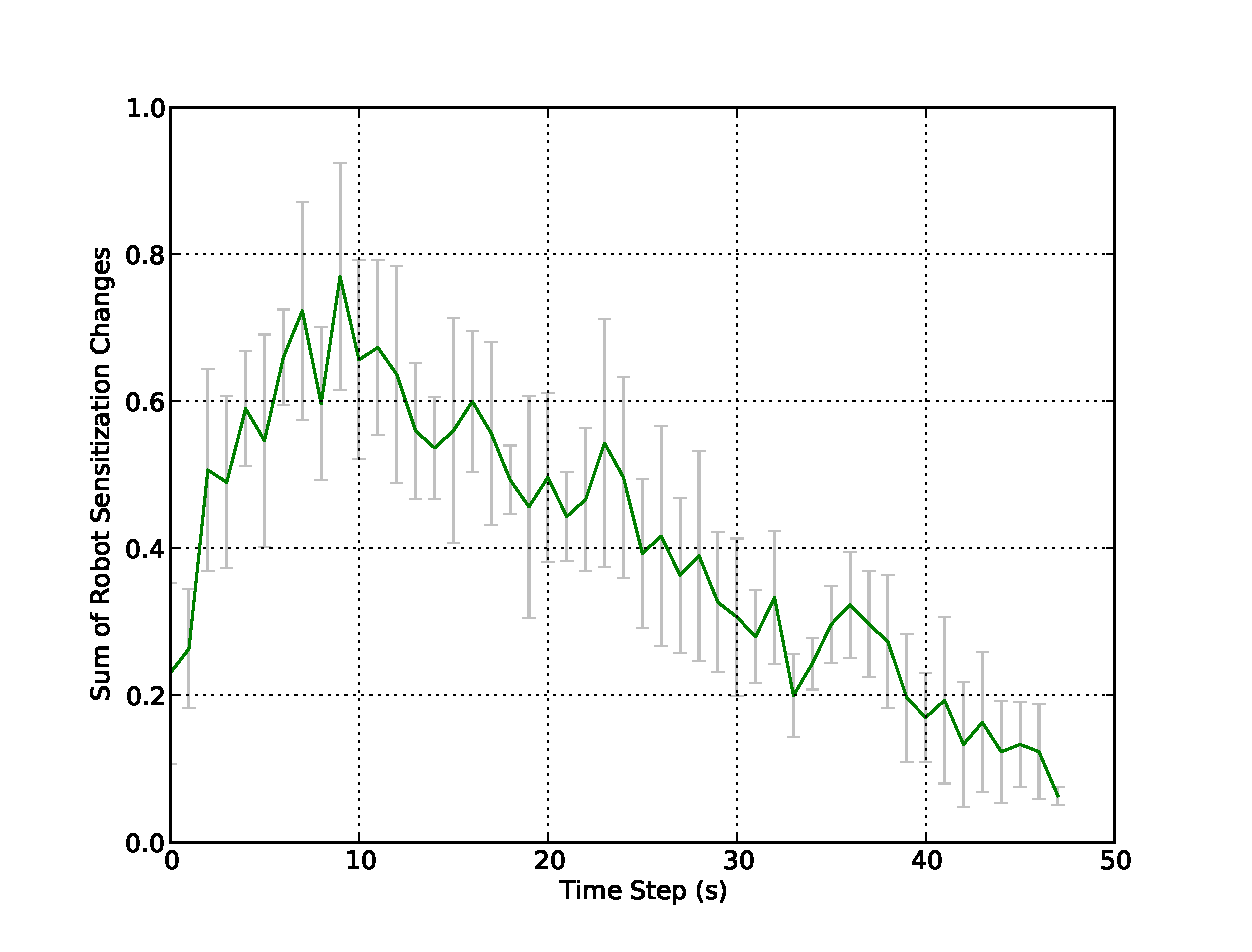
\includegraphics[height=5cm,width=3in]
{images/local-500cm/RobotSensitizationStat-Total-50steps}
%figure caption is below the figure
\caption{\small Changes in sensitizations  in local mode $r_{comm}$=0.5m}
\label{fig:local50cm-sensitization-stat} % Give a unique label
\end{minipage}
\hspace{0.5cm}
\begin{minipage}[t]{0.5\linewidth}
\centering
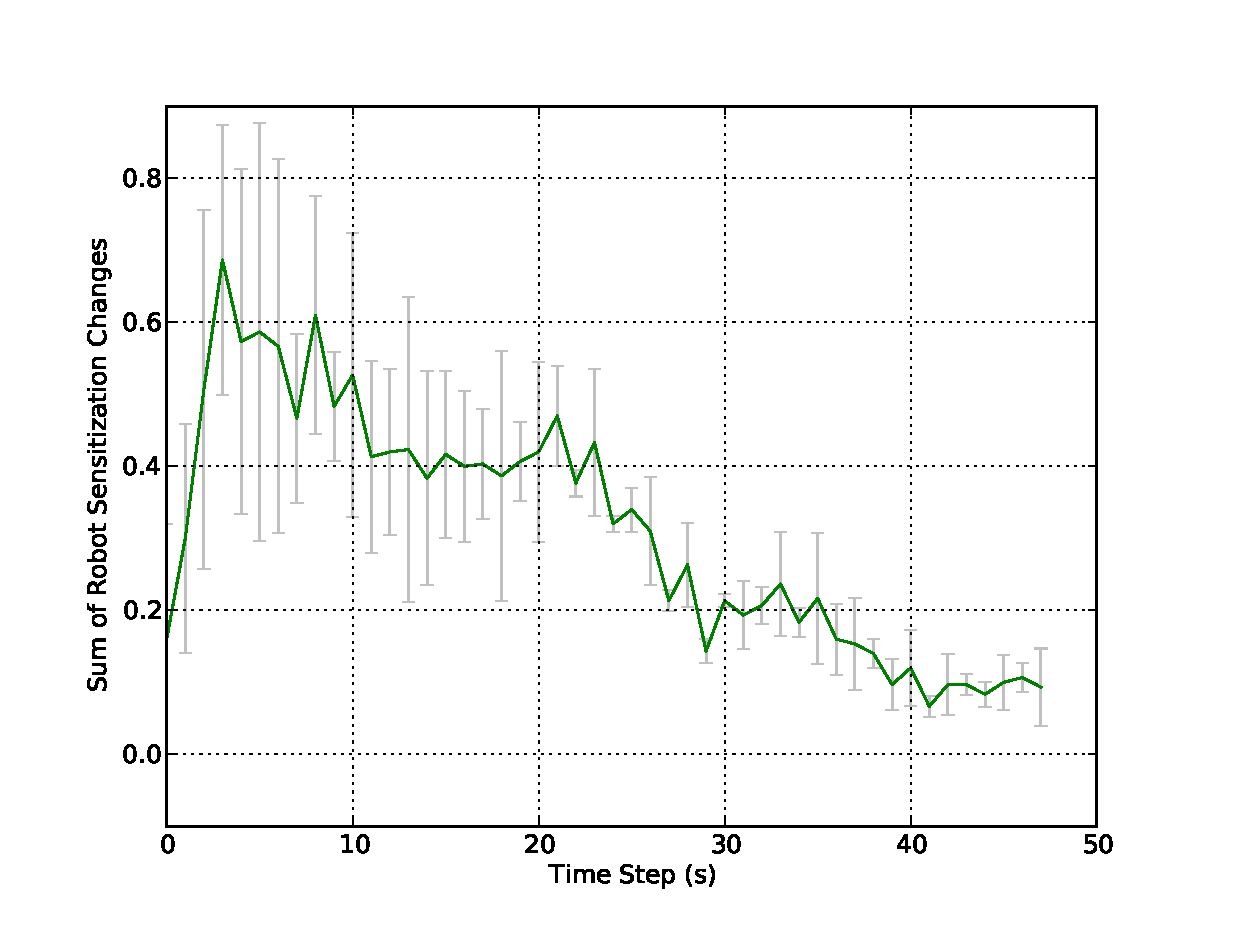
\includegraphics[height=5cm,width=3in]{images/local-1m/RobotSensitizationStat-Total-50steps}
\caption{\small Changes in sensitizations  in local mode $r_{comm}$=1m}
\label{fig:local1m-sz} % Give a unique label
\end{minipage}
\end{figure*}
%%
We have aggregated the changes in translation motion of all robots over time. Let $u_{i,q}$ and $u_{i,q+1}$ be the translations of a robot $i$ in two consecutive steps. If the difference between these two translations be $\delta u_{i}$, we can find the sum of changes of translations of all robots in $(q+1)^{th}$ step using the following equation.
\begin{equation}
\small 
\Delta U_{q+1} = \sum_{i=1}^{N} \delta u_{i, q+1} 
\label{eqn:Delta-Tr}
\end{equation}
The result from centralized communication experiment is plotted in Fig. \ref{fig:translation-stat}. In this plot we can see that robot translations also vary over varying task requirements of tasks. But it fails to show a consistence behaviour like previous plots. The robot translation results from local mode experiments are plotted in Fig. \ref{fig:local50cm-tr} and Fig. \ref{fig:local1m-tr}. The reduction of robot translation is significant in both local communication experiments.\\
%
%%% Sensitization
Similar to Eq. \ref{eqn:Delta-Phi}, we can calculate the absolute sum of changes in sensitizations by all robots in the following equation.
% 
\begin{equation}
\small 
\Delta K_{j, q+1} = \sum_{j=1}^{M} \left | \Delta k_{j, q+1} \right |
\label{eqn:Delta-K}
\end{equation}
This values of $\Delta K$ from local experiments are plotted in Fig.~\ref{fig:local50cm-sensitization-stat} and Fig.~\ref{fig:local1m-sz}. They show that the overall rate of learning and forgetting decrease over time. It is a consequence of the gradually increased task specializations of robots.\\
%%%% Single robot- number of peers
\begin{figure*}
\begin{minipage}[t]{0.5\linewidth}
\centering
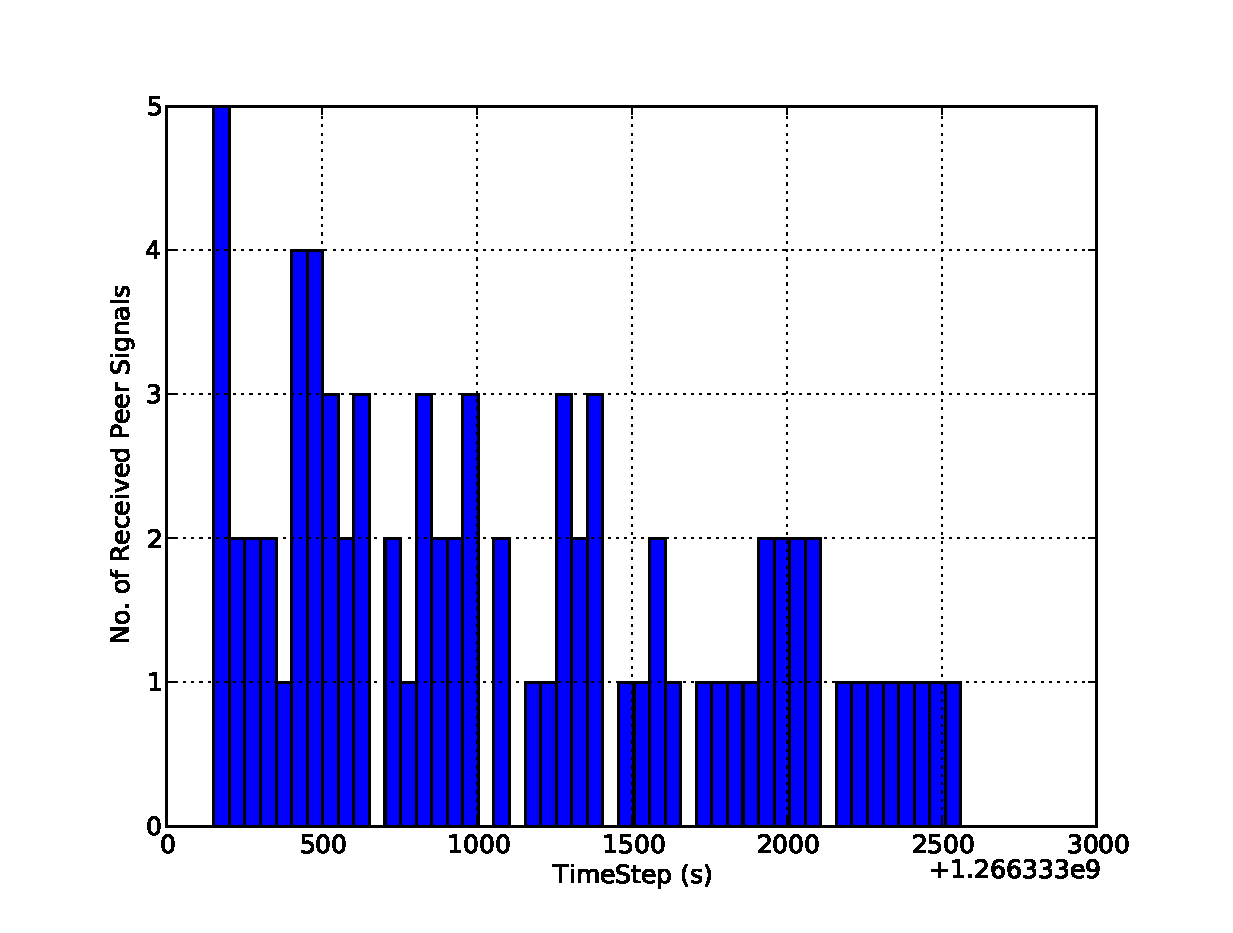
\includegraphics[height=5cm,width=3in]{images/local-500cm/Robot12-16feb-1-LocalSignals}
\caption{\small Peer signals caught by Robot12 in local mode $r_{comm}$=0.5m}
\label{fig:local50cm-single-robot-signal}% Give a unique label
\end{minipage} 
%%%
\begin{minipage}[t]{0.5\linewidth}
\centering
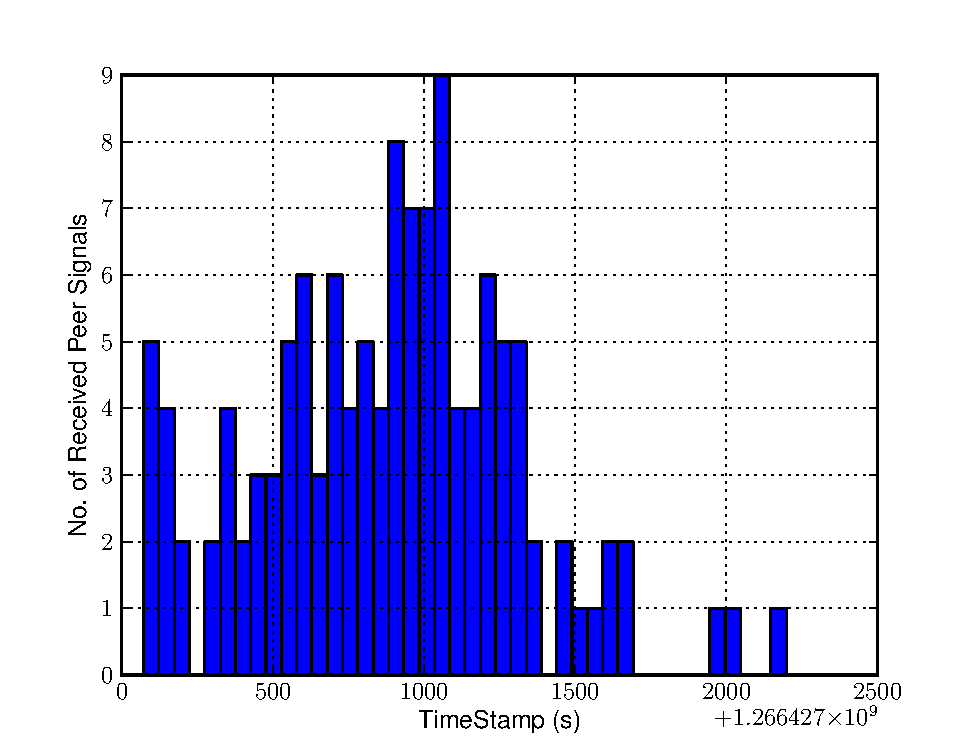
\includegraphics[height=5cm,width=3in]{images/local-1m/Robot12-17feb-3-LocalSignals}
\caption{\small Peer signals caught by Robot12 in local mode $r_{comm}$=1m}
\label{fig:local1m-single-robot-signal} % Give a unique label
\end{minipage}
\end{figure*}
%%% Communication load %%%
\begin{figure*}
\begin{minipage}[t]{0.5\linewidth}
\centering
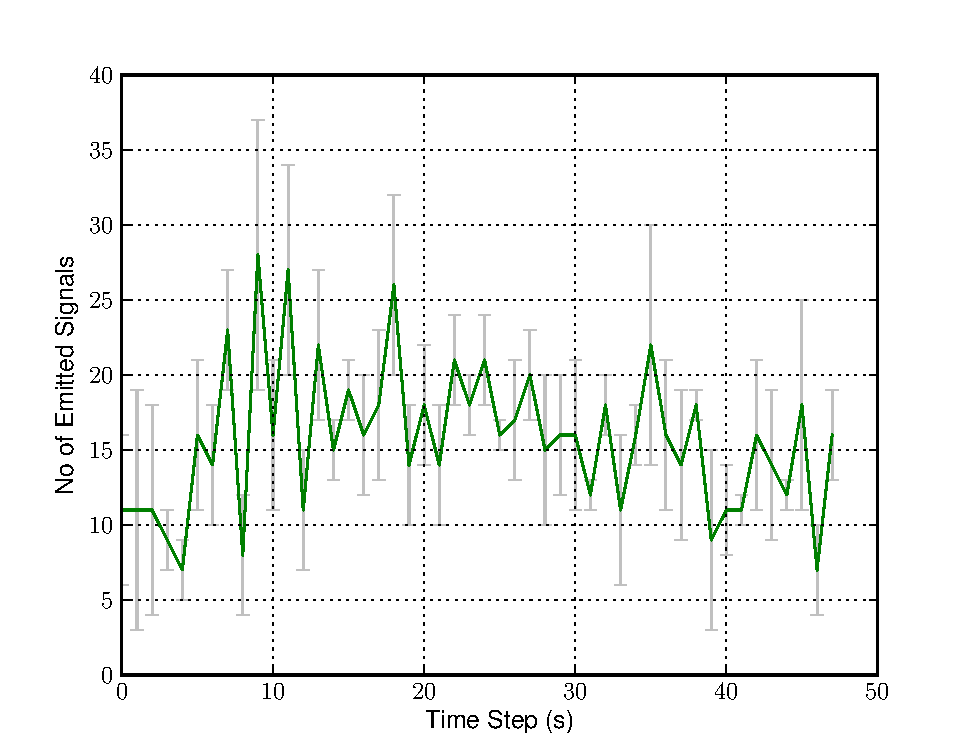
\includegraphics[height=5cm,width=3in]
{images/local-500cm/Local-500cm-SignalingFreqStat}
\caption{\small Frequency of P2P signalling in local mode $r_{comm}$=0.5m}
\label{fig:local50cm-signal-frequency-stat} % Give a unique label
\end{minipage}
\hspace{0.5cm}
\begin{minipage}[t]{0.5\linewidth}
\centering
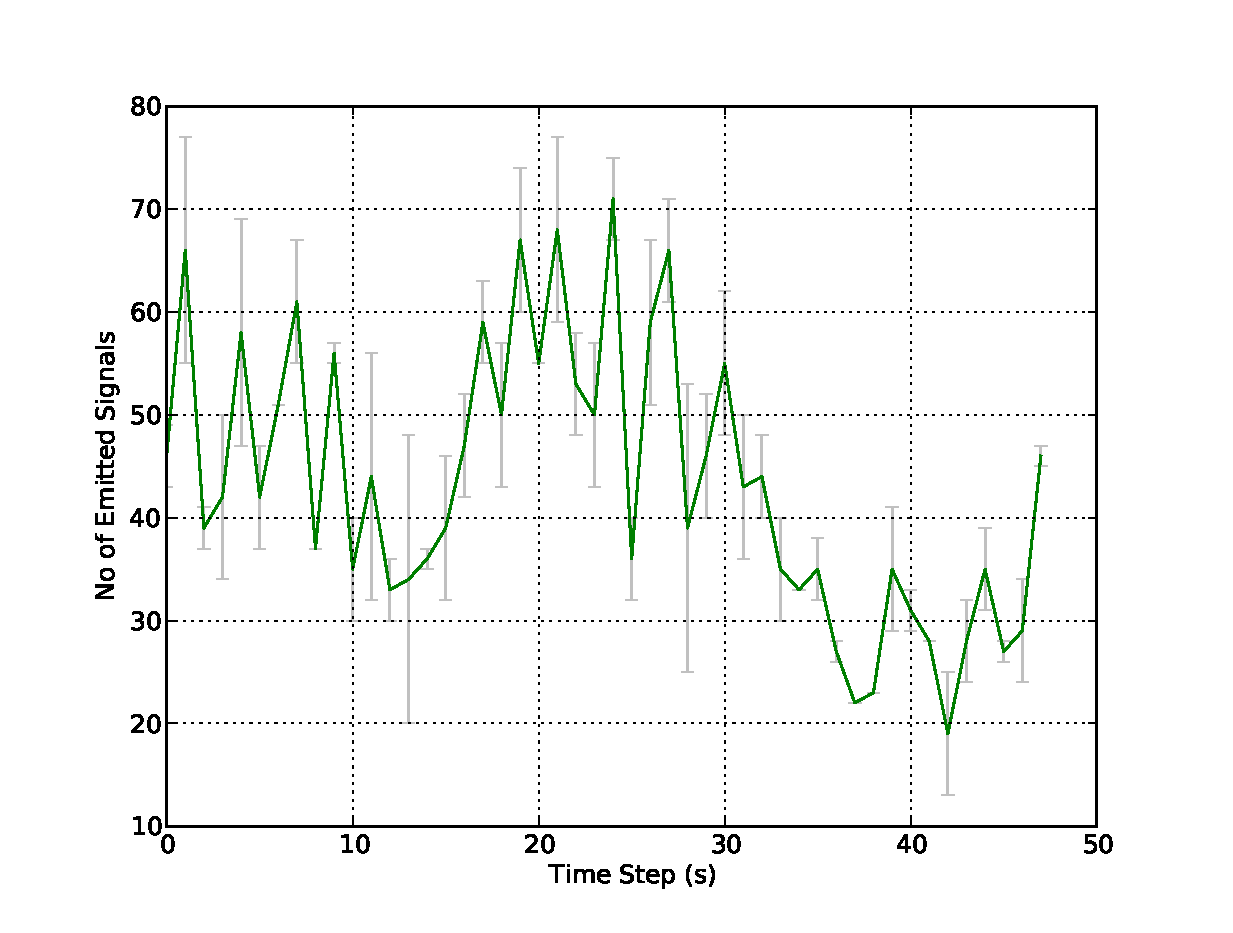
\includegraphics[height=5cm,width=3in]{images/local-1m/Local-1m-SignalingFreqStat}
\caption{\small Frequency of P2P signalling in local mode $r_{comm}$=1m}
\label{fig:local1cm-signal-frequency-stat} % Give a unique label
\end{minipage}
\end{figure*}
%
%%
As an example of P2P signal reception of a robot, Fig. \ref{fig:local50cm-single-robot-signal} and Fig. \ref{fig:local1m-single-robot-signal} show the number of received signals by Robot12 in two local experiments. It states the relative difference of peers over time in two local cases. The overall P2P task information signals of both of these local modes are plotted in Fig. \ref{fig:local50cm-signal-frequency-stat} and Fig. \ref{fig:local1cm-signal-frequency-stat}. Note that in centralized communication mode the task info signal frequency was kept 20 signals per time step \cite{Sarker}.\\ 
%%%% Single- robot sensitization and translation
\begin{figure*}
\begin{minipage}[t]{0.5\linewidth}
\centering
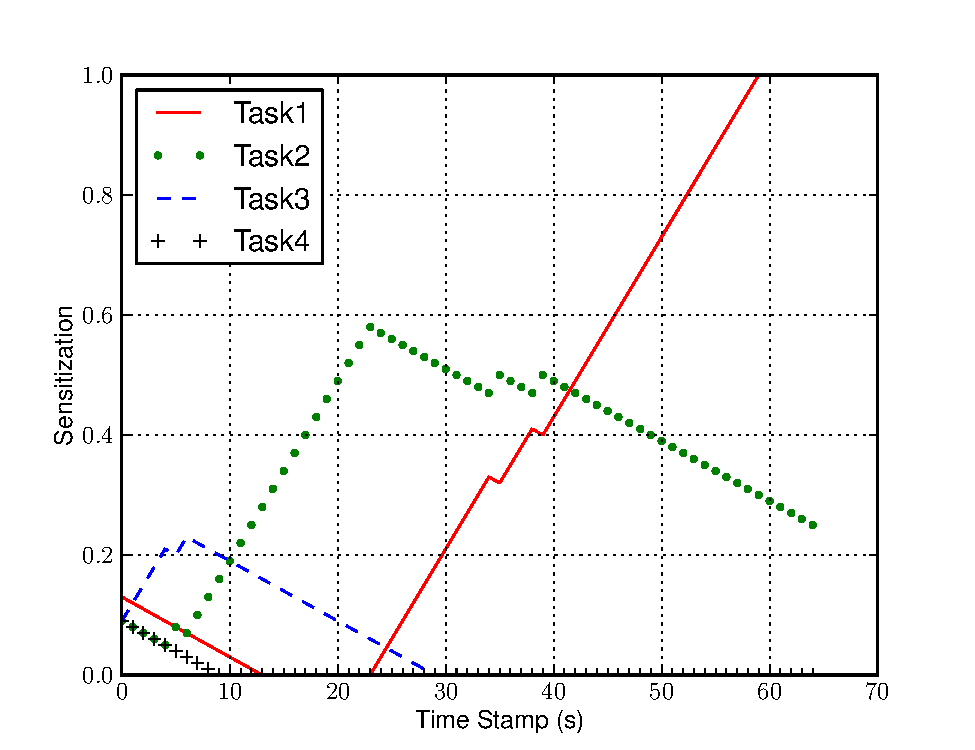
\includegraphics[height=5cm,width=3in]{images/local-500cm/PlotRobot12-Sensitizations-2010Feb16-150432}
\caption{\small Task specialization of Robot12 in local mode $r_{comm}$=0.5m}
\label{fig:single-robot-sensitizations} % Give a unique label
\end{minipage} 
%%%
\begin{minipage}[t]{0.5\linewidth}
\centering
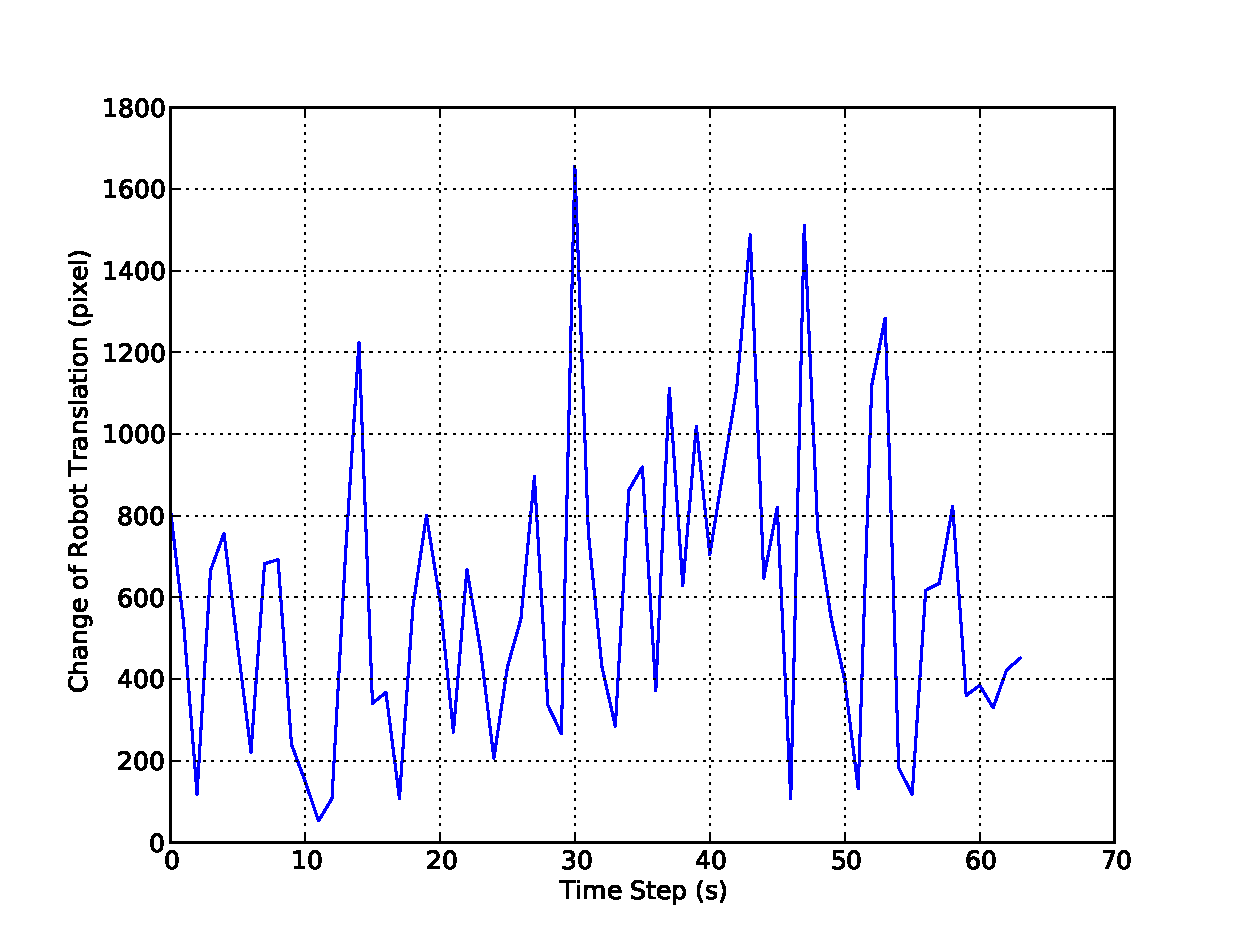
\includegraphics[height=5cm,width=3in]
{images/local-500cm/DeltaRobot12-PoseAtTS-2010Feb16-150432}
\caption{\small Changes in translation of Robot12 in local mode $r_{comm}$=0.5m}
\label{fig:single-robot-translation} % Give a unique label
\end{minipage}
\end{figure*}
%%%%
As an example of task specialization of a robot we plotted sensitization of Robot12 in Fig. \ref{fig:single-robot-sensitizations}. It shows that this robot has specialized in Task1. The continuous learning of Task1 happens from step 23 to step 59 where it has learned this task completely. This behaviour was found common in all robots with varying level of sensitizations. Hence we get the linear decrease of $\Delta K$ in sensitization plots. However, the changes in motion of this robot plotted in Fig. \ref{fig:single-robot-translation} was not stable due to the fact that robots frequently avoid dynamic obstacles and select random-walking.
%
%%%%%%%%%%%%%%%%%%%%%%%%%%%%%%%%%%%%%%%%%%%%%%%%%%%%%%%%%%%%%%%%%%%%%%%%%%%%%%%%
%%%%%%%%%%%%%%%%%%%%%%%%%%%%%%%%%%%%%%%%%%%%%%%%%%%%%%%%%%%%%%%%%%%%%%%%%%%%%%%%
\section{Related Works}
\label{sec:bg}
Krieger and Billeter presented MRTA in a team of 12 robots in ants' foraging scenario where a central server sent broadcast message containing energy level of the colony to all robots \cite{Krieger}. They also applied a form of indirect communication in order to share information about discovered food sources among robots. Although this P2P communication did not happen in real time, it improved the robustness of peer recruitment when compared with centralized communication only. Agassounon and Martinoli compared three task-allocation algorithms using simulations and reported that algorithm that used information sharing among local peers became robust in worker allocation \cite{Agassounon}. However, environment condition should be known {\em a priori} to optimize some parameters. By modulating the transmission power of local on-board wireless device of E-puck robots, Cianci {\em et al.} enabled them to communicate in different local radii \cite{Cianci}. In a self-organized decision making experiment, decision of 15 robots converged faster when local communication radius was relatively higher. Since the number of tasks was only two (left or right wall following), robots got global view of the system with increased communication radius. Thus they agreed quickly in one task.
%%%%%%%%%%%%%%%%%%%%%%%%%%%%%%%%%%%%%%%%%%%%%%%%%%%%%%%%%%%%%%%%%%%%%%%%%%%%%%%%
\section{CONCLUSIONS AND FUTURE WORKS}
\label{sec:conc}
We presented a locality based dynamic P2P communication model that achieves similar or better self-regulated multi-robot task allocation (MRTA) than its centralized counterpart. Particularly the reduction in robot movement states that local model is preferable when we need to minimize robot energy usage. Our model assumes no prior knowledge of the environment and it also does not depend on the number of the robots. We presented an abstract algorithm that can be used with various P2P communication technologies. We reported our implementation of this algorithm   by using  D-Bus technology in Linux. Comparative results from local mode experiments shows us that robots relatively perform better when the radius of communication is such small that most of the robots only communicate with their closest peers. This is contrary to the findings from \cite{Rutishauser, Epuck} where increased amount of information help to get desired task-allocation quickly. In our case, more information exchange with larger communication radius or with centralized communication increased task switching among robots. In case of local information exchange, robots have more chances to select local tasks by the virtue of self-regulating principles. Thus in local communication mode our system converged better and significantly reduced robot motions.\\ 
Our future work include performing more experiments with increased number of robots (up to 40) and tasks. Since our existing Bluetooth communication setup with one server fail to scale we are looking forward to distribute communication loads over a network cluster of tens of servers.
%%%%%%%%%%%%%%%%%%%%%%%%%%%%%%%%%%%%%%%%%%%%%%%%%%%%%%%%%%%%%%%%%%%%%%%%%%%%%%%%
\begin{thebibliography}{99}
\bibitem{Bonabeau+1999}
Bonabeau, E., Dorigo, M. and Theraulaz, G.:
Swarm intelligence: from natural to artificial systems.
Oxford University Press 1999
\bibitem{Labella}
Labella, T. H.; Dorigo, M. and Deneubourg, J. Division of labor in a group of robots inspired by ants' foraging behavior ACM Trans. Auton. Adapt. Syst., ACM, 2006, 1, 4-25
\bibitem{Elsa}
Arcaute, E.; Christensen, K.; Sendova-Franks, A.; Dahl, T.; Espinosa, A. and Jensen, H. J. : 
Division of labour in ant colonies in terms of attractive fields. 
Ecological Complexity, Elsevier 2008
\bibitem{SwisTrack}
Lochmatter T., Roduit P., Cianci C., Correll N., Jacot J., and Martinoli A.: 
SwisTrack - A Flexible Open Source Tracking Software for Multi-Agent Systems. 
In Proceedings of the IEEE/RSJ 2008 International Conference on Intelligent Robots and Systems (IROS 2008), pp 4004-4010
\bibitem{Epuck}
Cianci, C., Raemy, X., Pugh, J. and Martinoli, A.: Communication in a swarm of miniature robots: The e-puck as an educational tool for swarm robotics Swarm robotics: second SAB 2006 international workshop, Rome, Italy, September 30-October 1, 2006: revised selected papers, 2007, 103
\bibitem{Sarker}
Sarker M. O. F. and Dahl T. S.: Robotic Validation of an Inter-disciplinary Generic
Model of Self-regulated Division of Labour in Social Systems, ANTS 2010, 7th International Conference on Swarm Intelligence (submitted, available upon request).
\bibitem{Balch}
Balch, T. and Arkin, R. Communication in reactive multiagent robotic systems Autonomous Robots, Springer, 1994, 1, 27-52
\bibitem{Gerkey}
Gerkey, B. and Mataric, M. Principled communication for dynamic multi-robot task allocation Experimental Robotics VII, 2001, 353-362
\bibitem{Rutishauser}
Rutishauser, S.; Correll, N. and Martinoli, A. Collaborative coverage using a swarm of networked miniature robots Robotics and Autonomous Systems, Elsevier, 2009, 57, 517-525
\bibitem{Krieger}
Krieger, M. and Billeter, J. The call of duty: Self-organised task allocation in a population of up to twelve mobile robots Robotics and Autonomous Systems, Citeseer, 2000, 30, 65-84
\bibitem{Agassounon}
Agassounon, W. and Martinoli, A. Efficiency and robustness of threshold-based distributed allocation algorithms in multi-agent systems Proceedings of the first international joint conference on Autonomous agents and multiagent systems: part 3, 2002, 1090-1097
\bibitem{Mataric}
Mataric, M. Using communication to reduce locality in distributed multiagent learning Journal of experimental and theoretical artificial intelligence, 1998, 10, 357-369
%\bibitem{RobotTeam}
%Balch, T. and Parker, L. Robot Teams: From Diversity to Polymorphism, AK Peters, Ltd., 2002
\bibitem{Bluetooth}
Huang, A.S. and Rudolph, L.:
Bluetooth essentials for programmers.
Cambridge University Press 2007.
%\bibitem{c1}
%J.G.F. Francis, The QR Transformation I, {\it Comput. J.}, vol. 4, 1961, pp 265-271.
%
%\bibitem{c2}
%H. Kwakernaak and R. Sivan, {\it Modern Signals and Systems}, Prentice Hall, Englewood Cliffs, NJ; 1991.
%
%\bibitem{c3}
%D. Boley and R. Maier, "A Parallel QR Algorithm for the Non-Symmetric Eigenvalue Algorithm", {\it in Third SIAM Conference on Applied Linear Algebra}, Madison, WI, 1988, pp. A20.
\end{thebibliography}
\end{document}
